% $Id: gui_amodel.tex 395 2011-11-17 22:34:59Z cphillip $
%
% Written by A Marquand, updated by J. Schrouff for v2.0
%_______________________________________________

\chapter{Model Specification and Estimation}
\label{chap:ModelCrossV}
\minitoc

\section{Introduction}

The specification of a model is the core step of the pattern recognition pipeline and  entails setting up the combination of the different components making up the analysis. For example, model specification is where you select which data features to use as input (i.e. a feature set), the type of prediction to perform (e.g. classification or regression), which machine learning algorithm to employ (e.g. support vector machines, Gaussian processes, ...), which cross-validation strategy to employ (e.g. leave one subject out, leave one run out, ...) and which operations or manipulations to apply to the kernel before the algorithm is trained. The framework provided by PRoNTo is highly flexible and supports most types of pattern recognition analysis typically performed in neuroimaging. This chapter provides an overview of each of the components making up a model in PRoNTo. The presentation will focus on the user interface although it is important to note that the batch system provides several advanced options not available in the user interface (described further).

\section{Beginning a model specification}

To begin a model specification with the PRoNTo user interface, select `Specify model' from the main PRoNTo window. This will launch the model specification window (Figure \ref{fig_specify_model})

\begin{figure}[!h]
\begin{center}
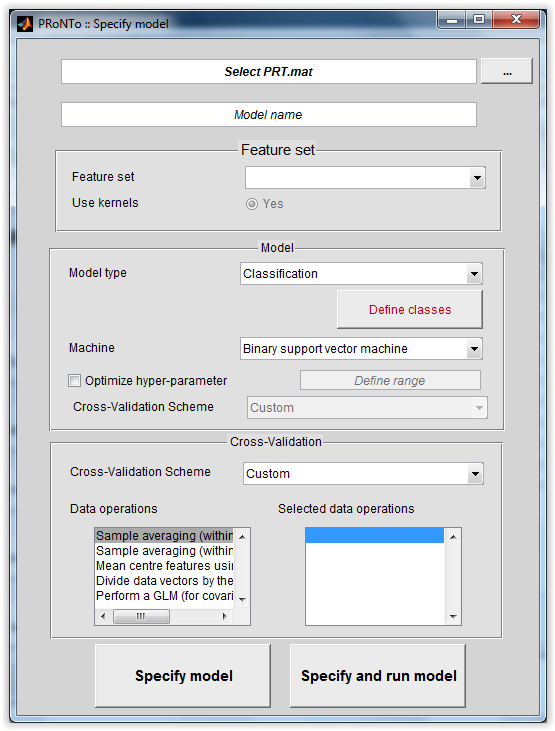
\includegraphics[height=3.5in]{images/prt_ui_model.png}
\caption{Model specification graphical user interface}
 \label{fig_specify_model}
\end{center}
\end{figure}

Next, select the \texttt{PRT.mat} containing your experimental parameters. Note that at least one feature set must be defined in this structure before a model can be created. See chapter \ref{chap:PrepFeat} for details on constructing feature sets.

Enter a unique name to identify the model, which is used internally in PRoNTo, by the batch system and for display purposes. It is a good idea to select a meaningful but short name (without spaces). \textbf{Note:} the \texttt{PRT.mat} data structure retains a permanent record of all models created but if a model with the specified name already exists in the \texttt{PRT.mat} data structure, it will be automatically overwritten.

\section{Feature set}
The drop-down list entitled `Feature set' will be populated once a \texttt{PRT.mat} containing one or more feature sets is selected. Select the appropriate feature set from the drop-down list. Note that a single feature set may contain more than one data modality (see chapter \ref{chap:PrepFeat}), which can be combined to build multimodal classification and regression models (e.g. L1-Multiple Kernel Learning models). This might also be useful if more than one run/session is available for each subject, in which case each run could be input as an independent modality in the data and design step and a single-subject classifier might be specified using leave-one-run-out cross-validation. 

In the current release of PRoNTo, only kernel machines are supported via the user interface. The capability to support non-kernel techniques will be added in a future release. Thus, the `Use kernel' radio button should always be set to true.

\section{Model type / pattern recognition algorithm}
In this part of the model specification input form, select the pattern recognition algorithm to employ (referred to in PRoNTo as a `machine'). In the current release, three classification algorithms are supported (binary support vector machines, Gaussian processes (binary and multiclass) and L1-Multiple Kernel Learning) and four multivariate regression methods (Gaussian process regression, kernel ridge regression 
\footnote{Kernel ridge regression is equivalent to a \emph{maximum a posteriori} approach to Gaussian process regression with fixed prior variance and no explicit noise term} , relevance vector regression and L1-Multiple Kernel Learning). 

\textbf{Note:} if a feature set contains multiple kernels (either from regions of interest or based on different modalities) but the selected classification/regression technique is a single kernel method (e.g. SVM or KRR), the kernels will first be summed before entering the classification/regression phase. This corresponds to concatenating the features before building the kernel. For regions of interest in a single modality, the summed kernel is hence equivalent to a whole brain model.

The PRoNTo user interface provides a mechanism for flexible definition of which components of the data design should be used for each classification or regression model. Note that this will not necessarily be the whole experiment; for example, in a complex fMRI experiment there may be several groups, each containing multiple subjects, each in turn having multiple experimental conditions (e.g. corresponding to
different subprocesses of a cognitive task). In such cases, it is usually desirable to ask several different questions using the data, such as discriminating between groups for a given experimental condition (``between group comparison"), discriminating between experimental conditions for a fixed group (`between-task comparison') or training independent pattern recognition models for different subsets of subjects. All of
these can be easily defined via the user interface by clicking the `Define classes' button (for classification) or `Select subjects/scan' (for regression).

\subsection{Classification}

The class selection panel is displayed in figure \ref{fig_specify_classesC}. First, define the number of classes, noting that some classification algorithms (e.g. support vector machines) are limited to binary classification, while other classification algorithms (e.g. Gaussian processes) support more than two classes. Enter a name for each class - again, it is a good idea to make these names informative but short. Notice that immediately after the number of classes has been specified, the group-, subject- and condition selection panels are greyed out. To enable them, simply select one of the classes from the drop-down menu.

For each class, select the subjects and conditions (if any) that collectively define that class. It is possible to select multiple experimental
conditions in the same class, but this complicates model interpretability and potentially also model performance (since by definition
conditions are not identically distributed). If a condition or subject is erroneously selected, click on it in the `selected subject(s)' or
`selected condition(s)' panel and it will be removed from the list. The performance of classification models is evaluated based on measures such as total accuracy, class accuracies and positive predictive values (representing the sensitivity and specificity). 

\begin{figure}[!h]
\begin{center}
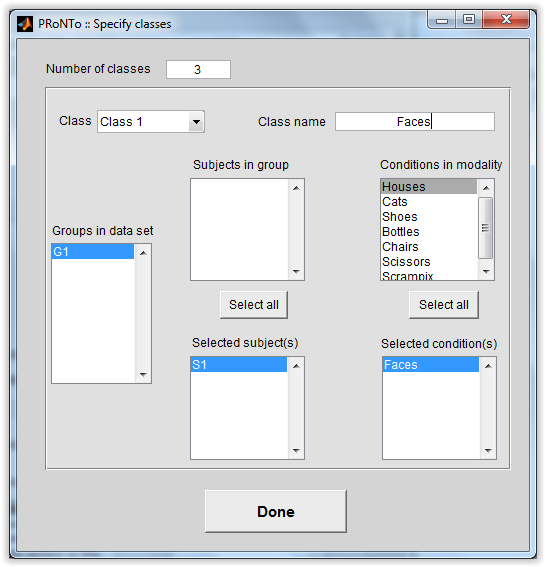
\includegraphics[height=3.5in]{images/prt_ui_model_classes.PNG}
\caption{Subject / condition selection panel for classification models}
 \label{fig_specify_classesC}
\end{center}
\end{figure}

\subsection{Regression}

Regression is a generic term for all methods attempting to fit a model to observed data in order to quantify the relationship between two groups of variables. Traditionally in neuroimaging massively univariate strategies (e.g. GLM) have been largely used, where data for each voxel are independently fitted with the same model. Statistics test are used to make inferences on the presence of an effect at each voxel (e.g. \emph{t-test}).  Multivariate regression, on the other hand, takes into account several input variables (voxels) simultaneously, thus modelling the property of interest considering existing relations among the voxels.

Although most studies exploring predictive analyses in neuroimaging have been related to classification, regression analysis has aroused interest in neuroscience community for its ability to decode continuous characteristics from neuroimaging data. This approach has potential to be used when the examples (patterns) can be associated to a range of real values. The objective is to predict a continuous value instead of predicting a class to which the example belongs. These values usually refer to demographic, clinical or behavioural data (as age, blood pressure or scores resulting from a test, for example). For validation, different metrics can be used to compute the agreement between the predicted values and the actual ones, such as Pearson's correlation coefficient (r) and Mean Squared Error (MSE).

The specification of which subjects and scans to include in regression models is similar to that for classification, see Figure  \ref{fig_specify_classesR} and for the purposes of model specification in PRoNTo, regression can be thought of as a classification problem with a single class. In the current release, regression is only supported if there is a single scan per subject (e.g. structural images or beta images from a GLM analysis). In a future release it will be possible to perform regression where an independent regression target is supplied for each trial, block or condition. To perform a regression, the regression targets are specified during the design stage. It is important to emphasize that in the current implementation, regression is only supported using the "select by scans" option (see chapter \ref{chap:DataDesign}).  

\begin{figure}[!h]
\begin{center}
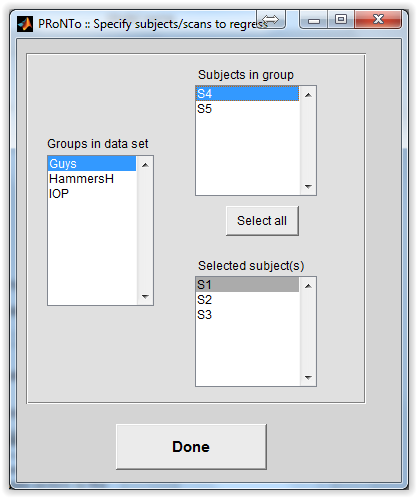
\includegraphics[height=3.5in]{images/prt_ui_model_regression.PNG}
\caption{Subject / condition selection panel for regression models}
 \label{fig_specify_classesR}
\end{center}
\end{figure}

\subsection{Hyper-parameter optimization}

From PRoNTo version 2.0, it is possible to optimize hyper-parameters of the machine learning models. For example, the soft-margin (a.k.a. C) hyper-parameter in
SVM can be optimized, using a nested cross-validation scheme. In this case, there are two loops in the cross-validation scheme. The inner loop is used for parameter optimization and the outer loop is used for assessing the model's performance. More specifically, the data is divided into training and testing sets according to the cross-validation scheme selected (outer loop). For each fold of the outer loop the training set is further divided into training and testing sets according to the cross-validation scheme selected (inner/nested loop). The inner loop is used to train and test the model with each value of the hyper-parameter specified by the user. The parameter leading to the highest performance in the inner/nested loop (balanced accuracy for classification and Mean Squared Error for regression) is then used in the outer loop. For each fold of the outer loop, the model is trained using the 'optimal' value of the hyper-parameter and tested on the data that was left out (and which was not used for parameter optimization). This nested CV procedure can lead to different values of the hyper-parameter to be selected in each fold. These are stored in the outputs of the model and can be reviewed in the `Display Results' panel.

Optimizing the hyper-parameter might lead to improved results compared to fixed values. This will usually depend on the number of features selected to model the data: for example, for whole brain models based on SVM classifiers, with many more features than images/trials, it is reasonable to assume that changing the hyper-parameter won't affect the model performance significantly due to the high dimensionality of the data with respect to the number of examples. However, when using (e.g.) regions of interest (in a second-level mask or in a MKL model), the ratio between the number of features and the number of examples will be much smaller. In this case, different values of the hyper-parameter might lead to different decision functions and optimizing the hyper-parameter is desirable.

Performing a nested cross-validation can be computationally expensive. For computational efficiency, PRoNTo allows to specify different cross-validation schemes for the `outer' and the `nested' CV\footnote{For example, the outer CV could have more folds, to use as much data as possible in each fold for prediction (e.g. leave-one-out), while the nested CV would not need as many folds to select the `optimal' value of the hyper-parameter (e.g. k-folds CV).}. 

In the current version of PRoNTo, the soft-margin parameter can be optimized for SVM and for MKL (classification and regression). In the same way, it is possible to optimize the $\lambda$ ridge parameter for KRR. If no value is provided, those parameters will take the values $0.01, 0.1, 1, 10, 100$ and $1000$, i.e. $10.^{[-2:3]}$.

\section{Cross-validation}

In the final part of the specify model input form, select the type of cross-validation to employ. Cross-validation is a crucial part of the
pattern recognition modelling and is used to assess the generalisation ability of the model and to ensure the model has not overfit to the data. Typically this is done by
partitioning the data into one or more partitions: a `training set', used to train the model (e.g. fit parameters) and a `testing set' used to assess performance on unseen data. By repeatedly repartitioning the data in this way, it is possible to derive an approximately unbiased estimate of the true generalisation error of the model. 

The most common cross-validation schemes in neuroimaging applications are leave-one-subject out (LOSO; exclude one subject for testing, train with the remaining), leave-one-run-out (LORO; leave one fMRI run out for testing, train with the remainder) and leave-one-block-out (LOBO; leave out a single block or event and train with the remainder). LOSO is suitable for multi-subject designs, while LORO and LOBO are suitable for single subject designs, where the former is better suited to designs having multiple experimental runs and the latter is appropriate if there is only a single run. The current release of PRoNTo supports each of these, and also supports leave-one-subject-per-group-out (LOSGO), which is appropriate if the subjects in each group are paired or for repeated measures experimental designs. Versions 1.1 and later allows k-fold cross-validation for each of the available schemes. This means that the user specifies the number of folds (`k') and that the data is partitioned according to that number. For example, specifying $k=4$ will use 25\% of the data to test the model, and 75\% to train it. Note: $k=1$ splits the data in half, training the model on the first half and testing on the second, i.e. there is no circular partitioning.

In version 2.0, a GUI allows the user to fully specify his/her cross-validation scheme. First, a `basis' needs to be specified (Figure \ref{fig_customCV_basis}). Three options are available: 

\begin{itemize}
\item Load a .mat containing a previously computed CV matrix (needs to contain the variable `CV').
\item Select a basis from the pop-down list (contains the same options as for the outer CV).
\item Specify the number of folds.
\end{itemize}


\begin{figure}[!h]
\begin{center}
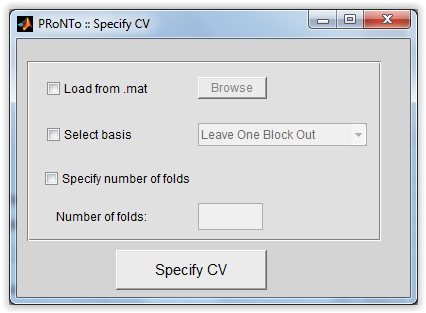
\includegraphics[height=4cm]{images/prt_customCV_basis.PNG}
\caption{Specify basis to build custom cross-validation}
 \label{fig_customCV_basis}
\end{center}
\end{figure}

When an option has been selected, a new window will appear (Figure \ref{fig_customCV}). The top panel of this window is a table that can be edited. Each row refers to a trial/image selected in the definition of the classes (or to perform regression on). Each column represents a fold. For each column, the different trials can have a value of 2 (test set), 1 (train set) or 0 (unused in this fold). Setting a whole fold to 0 takes it out of the CV matrix. Note: it is possible to change the value of multiple trials by changing the value of the last trial to modify, then shift-select the first one to modify. This also works across folds. The bottom panel displays the structure of the data selected for further classification or regression, along with a preview of the built CV matrix.

\begin{figure}[!h]
\begin{center}
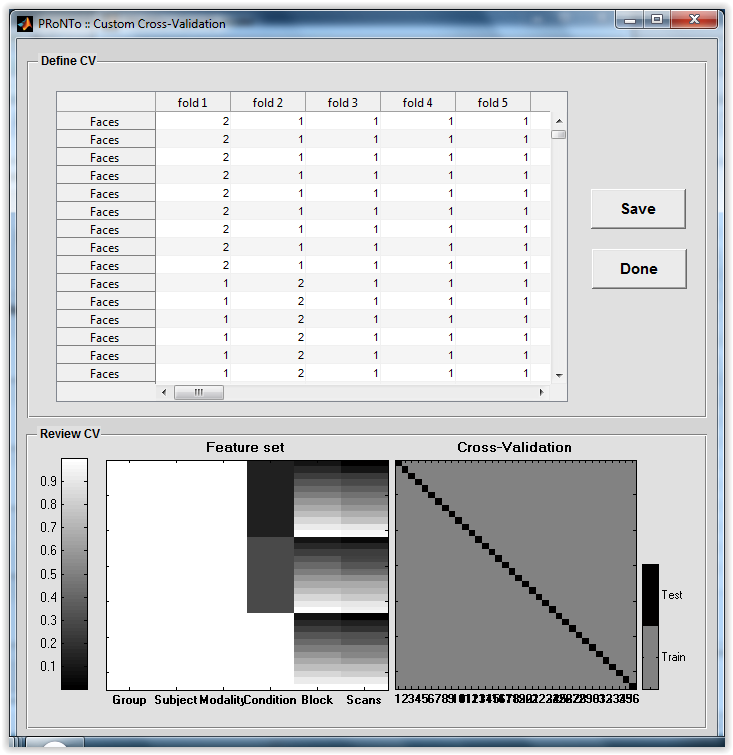
\includegraphics[height=9cm]{images/prt_customCV.PNG}
\caption{For each fold, specify which images/trials are part of the training and test set, or are unused}
 \label{fig_customCV}
\end{center}
\end{figure}

The resulting CV matrix can be saved in a .mat, alongside the PRT (name: \textit{model name\_ CV.mat}). This matrix can loaded as a custom CV in the batch, if exactly the same trials were selected for modelling. \textbf{Note:} The `custom' CV option is not available as a nested/inner cross-validation scheme. 

Information concerning the cross-validation structure is stored internally in matrix format, and can be visualised by clicking `Review Kernel and CV' from the main ProNTo window (see \ref{fig_reviewCV} for an example). In the left panel, this figure indicates which group, subject, modality and condition each scan in the feature set belongs to. On the right, each cross-validation fold (partition) is displayed as a separate column and each scan is colour coded according to whether it is in the training or testing set (or if it is unused).


\begin{figure}[!h]
\begin{center}
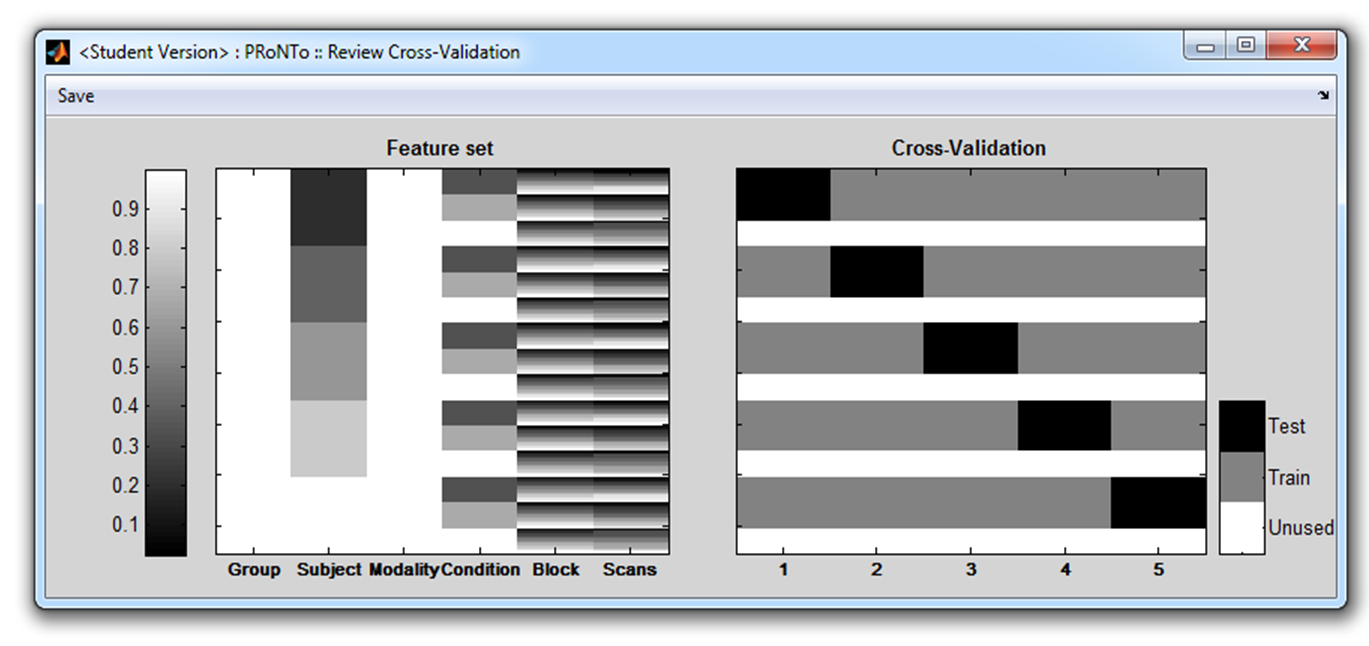
\includegraphics[height=2in]{images/prt_ui_reviewCV.png}
\caption{Review cross-validation matrix}
 \label{fig_reviewCV}
\end{center}
\end{figure}

It should be emphasised that the type of cross-validation selected should be appropriate for the experimental design. For example, it is nonsensical to select a leave-one-subject-out cross-validation approach for single subject designs. It is also important to ensure that the training and testing sets are completely independent to avoid the cross-validation statistics becoming biased. This is particularly important for fMRI, where successive scans in time are highly correlated. For example, if a leave-one-block-out approach is employed and the blocks are too close together then the independence of the training and testing set will be violated, and the cross-validation statistics will be biased (technically this is governed by the autocorrelation length of the fMRI timeseries and the temporal blurring induced by the haemodynamic response function). This can be avoided if care is taken to ensure that overlapping scans are discarded from the design (see chapter \ref{chap:DataDesign}), but it is a very important issue, and the user should still be careful to ensure that cross-validation folds are sufficiently far apart in time (especially for LOBO cross-validation).

During this part of the model specification, it is also possible to select one or more operations to apply to the data. Each of these operations is defined below:

\begin{enumerate}
\item \textbf{Sample averaging (within blocks):} constructs samples by computing the average of all scans within each block or event for each subject and condition. 
\item \textbf{Sample averaging (within subjects):} constructs samples by computing the average of all scans within all blocks for each subject and condition.
\item \textbf{Mean centre features using training data:} subtract the voxel-wise mean from each data vector.
\item \textbf{Divide data vectors by their norm:} scales each data vector (i.e. each example) to lie on the unit hypersphere by dividing it by its Euclidean norm.
%\item \textbf{Regressing out covariates:} regresses out the covariates entered for each subject/image (entered `by scans') from the kernel. \textbf{Note:} This operation is actually performed without taking into account the separation between training and test sets. A new formulation of this operation, taking into account the division of train and test, is currently in development and will be implemented as soon as possible.
\end{enumerate}


%(except for the GLM)
A crucial point to note is that all operations are embedded within the cross-validation structure such that they are applied independently to training and testing sets. This prevents a very common mistake in pattern recognition from occurring, whereby parameters are computed using the whole data set prior to cross-validation. Observing a complete split between training and testing sets during all phases of analysis ensures that accuracy measures are an appropriate reflection of the true generalisation ability of the machine and are not biased because of improper applications of preprocessing operations to the entire dataset.

Other points to note include: (i) the order of operations is potentially important. For example, subtracting the mean then dividing each data vector by its norm is not the same as performing the operations the other way around. (ii) operations (1) and (2) have no effect if no design is specified or for events with a length of one TR.

At a minimum, we recommend that features should be mean centered over scans during cross-validation. In addition, for multiple kernel learning, we advise the user to normalize each kernel. This will compensate for the fact that different kernels might be computed from examples/samples with different number of features (e.g. different regions contain different numbers of voxels).

The different operations selected for a specific model can then be reviewed using the `Review Kernel and CV' (starting from version 2.0). The selected operations will be listed below the kernels (`Show kernel').

\section{Specify / Run model}

Using the GUI, it is possible to either `Specify' the model, or `Specify and Run' the model. The first option saves all the parameters of the model in the PRT structure. This information can be found in \texttt{PRT.model(\textit{m}).input}, where \textit{m} is the index of the model. The second saves all the parameters of the model and then runs the model. In this case, the inputs, which include the cross-validation matrix, the target values or labels, and the machine (e.g. binary SVM, Gaussian Process, etc.), are fed to the estimation routines, which will then add to the PRT an output field (\texttt{PRT.model(\textit{m}).output}) containing the estimated parameters, statistics, and other information from the learning process.

In some cases (e.g. multiple models to run or models with nested CV and/or slower machines), it would be desirable to estimate models later on (e.g. just before lunch break or at the end of the day). The `Run model' option allows to select multiple models and run them one at a time automatically (Figure \ref{fig_run_model}). The first thing that needs to be done using this window is to specify which PRT we would like to work with. PRoNTo will then read the available models from this structure and display the list of models on the left panel. These models can be selected (the selected models will show on the right panel) by clicking each model individually or by clicking the `Select all' button in the middle of the panels. Finally, to estimate the model(s), one needs only to click the bottom button `Run model(s)'.

\begin{figure}[!h]
\begin{center}
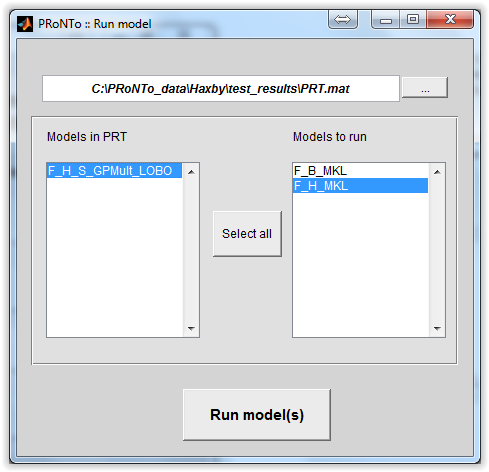
\includegraphics[height=5cm]{images/prt_run_model.PNG}
\caption{Choose models to be estimated}
 \label{fig_run_model}
\end{center}
\end{figure}

It is useful to have a look at what is displayed in the \matlab command space when the model is being estimated. Information such as the number of folds can help double-check that everything is going as expected. Furthermore, if some options were specified (e.g. using a feature set with multiple kernels) that are not available at the modelling step (e.g. to be modelled with SVM), warnings will be displayed, as in Figure \ref{fig_ws_matlab}.

\begin{figure}[!h]
\begin{center}
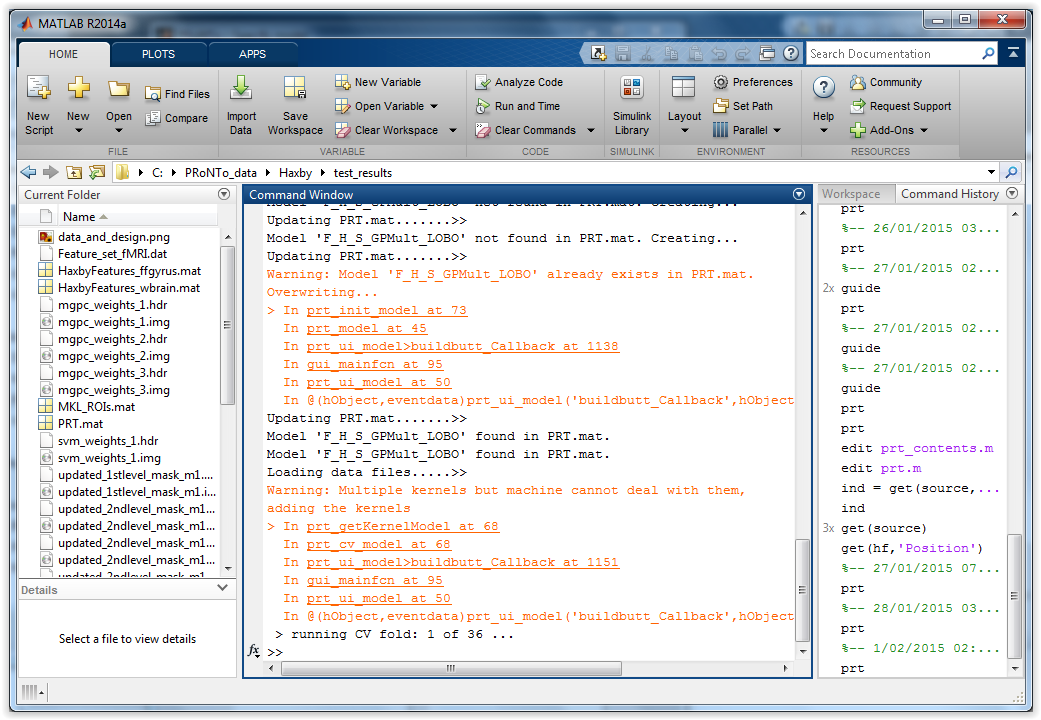
\includegraphics[height=8cm]{images/matlab_workspace_model.PNG}
\caption{\matlab workspace displaying warnings when kernels are added}
 \label{fig_ws_matlab}
\end{center}
\end{figure}

\textbf{Important note:} multiple kernel feature sets can be modelled using any machine. For machines not supporting multiple kernels, these will first be added before the model is estimated. This corresponds to concatenating the features from the different regions and/or modalities.

\section{Batch interface}

The batch module provides all the functionality provided in the user interface and allows complex analyses to be scripted in advance. As noted,
the batch module also provides functionality not available in the user interface. The most important difference is that the batch module allows
customised \matlab \ functions to be used as prediction machines. This functionality allows PRoNTo to be easily extended to allow many types of
classification and regression algorithms not provided under the current framework. This can be achieved by selecting `Custom machine' under the
`Model Type' heading. This allows a function name to be specified (i.e. any \texttt{*.m} function in the \matlab \ search path). The behaviour of this custom machine can then be controlled by a free-format argument string. See the developer documentation and the examples in the \texttt{machines/} subdirectory of the PRoNTo distribution for more information. Another important difference between the batch and user interfaces is that mean centering data vectors across scans is enabled by default in the batch. Also, flexible CV is available in the batch only in the form of `load a .mat'. This .mat must contain a variable called `CV', specifying the CV matrix for the selected trials/images.

An example of the batch window for model specification is provided in figure \ref{fig_batch_model}.

\begin{figure}[!h]
\begin{center}
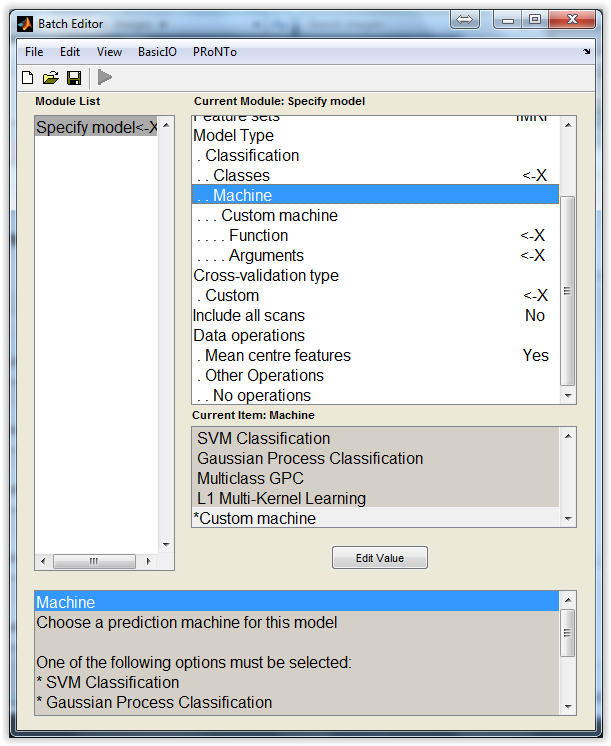
\includegraphics[height=3.5in]{images/prt_batch_model.PNG}
\caption{Batch interface to specify a model}
 \label{fig_batch_model}
\end{center}
\end{figure}

As displayed in Figure \ref{fig_batch_model}, the batch does not allow to specify and run the model directly. Instead, the user had to add a `Run model' module. The batch has the advantage of allowing to perform permutations along model estimation (option available in the `Display results' window in the GUI). Furthermore, it is possible to save the predictions and the balanced accuracy (for classification) for each permutation, to perform further statistical tests if needed. The `Run model' batch module is presented in Figure \ref{fig_batch_runmodel}. \textbf{Note:} Dependencies on the model name are available when performing a `Model specification' followed by a `Run model' module.

\begin{figure}[!h]
\begin{center}
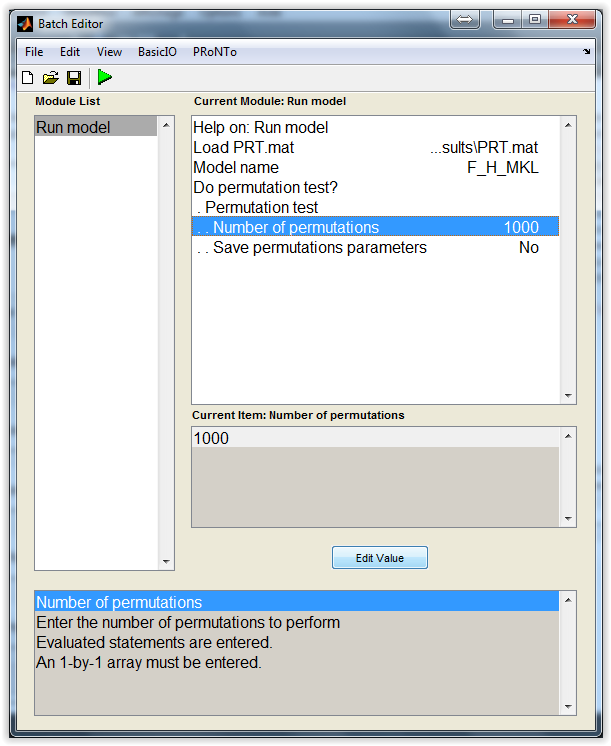
\includegraphics[height=3.5in]{images/prt_batch_runmodel.PNG}
\caption{Batch interface to run a model}
 \label{fig_batch_runmodel}
\end{center}
\end{figure}

